%%%%%%%%%%%%%%%%%%%%%%%%%%%%%%%%%%%%%%%%%%%%%%%%%%%%%%%%%%%%%%%%%
% Dissertacao de Mestrado / Dept Fisica, CFM, UFSC              %
% Lacerda@UFSC - 2013                                           %
%%%%%%%%%%%%%%%%%%%%%%%%%%%%%%%%%%%%%%%%%%%%%%%%%%%%%%%%%%%%%%%%%

%:::::::::::::::::::::::::::::::::::::::::::::::::::::::::::::::%
%                                                               %
%                          Capítulo 2                           %
%                                                               %
%:::::::::::::::::::::::::::::::::::::::::::::::::::::::::::::::%

%***************************************************************%
%                                                               %
%                      CALIFA & PyCASSO                         %
%                                                               %
%***************************************************************%

\chapter{O projeto CALIFA e o {\em pipeline} PyCASSO}
\label{sec:CALePyC}

As observações do universo modificaram completamente o nosso modo de viver,
pensar, compreender-se. Aprendemos a contar os dias, desenvolvemos um sistema
de meses, estações do ano, movimentos das marés, entre outras coisas que já são
parte do senso comum, mas que um dia foram o estado da arte da ciência. É assim
que surge o CALIFA: um projeto que está modificando nossa maneira de ver e
pensar as galáxias no nosso universo de forma que entendamos melhor a nossa também.

Com a massiva quantidade de dados obtidos, resultado direto de um projeto de
ciência de ponta, vem também a dificuldade da interpretação dos dados. No caso
do CALIFA, através da {\em pipeline} PyCASSO \citep{CidFernandes2013a}, a
programação investigativa se torna simples e ao mesmo tempo robusta,
facilitando a construção de todo tipo de resultados, sejam eles \ojo matemáticos
ou físicos.

%***************************************************************%
%                                                               %
%                            CALIFA                             %
%                                                               %
%***************************************************************%

\section{O survey CALIFA}
\label{sec:CALePyC:Apresent}

\ldots
Descrição básica. Figuras dos papers para exemplos de espectros, imagens e 
produtos do PyCASSO. Citar que usamos o COMBO (V500 + V1200).
\ldots

No sul da Espanha, mais precisamente em {\em Sierra de Los Filabres}
(Andalucía), está situado o germano-espânico {\em Calar Alto Observatory}. O
projeto CALIFA está sendo possível através de observações de o maior de seus
$3$ telescópios ($3.5$m) e terá ao todo $\sim600$ objetos ao longo de $250$
noites de observação. Em comparação com o \SDSS, o CALIFA terá a mesma ordem de
número de espectros para estudo, mas, apesar de um número menor de galáxias,
graças ao IFU será o com melhor completeza por objeto. Existem alguns poucos
surveys IFU e todos com, além de poucos objetos e FoV menor, focos de estudo
muito estreitos, dificultando o legado do survey para outras pequisas
científicas mais abrangentes \citep[SAURON; ][região central de 72 galáxias
com $z < 0.01$.]{de-Zeeuw2002} \citep[PINGS; ][algumas galáxias muito próximas
($\sim10$ Mpc) e o estudo atual de 70 (U)LIRGs com $z <0.26$]{RosalesOrtega2010}
\citep[VENGA; ][$30$ galáxias espirais]{Blanc2010}. Apesar de ser primariamente
construído para o estudo da física bariônica da evolução de galáxias, o CALIFA
está projetado para que seu legado seja bem abrangente, possibilitando diversos
tipos de estudos em diversas áreas.

\subsection{A ``{\em colméia}'' de fibras}

Neste telescópio basilar para o projeto CALIFA está instalado o equipamento
Potsdam Multi Aperture Spectrograph \citep[PMAS; ][]{Roth2005} no modo PPAK
\citep{Verheijen2004, Kelz2006} formando um espectrofotômetro de campo integrado
com um {\em bundle} de $382$ fibras (figura \ref{fig:BundlePPAK}), das quais,
$331$ são para observação dos objetos, outras $36$ para \ojo
\textcolor{blue}{sky background sample} e outras $15$ para calibração. As {\em
science fibers} ($331$) cobrem um {\em FoV} ({\em field-of-view}) hexagonal de
$74" X 64"$ que, através de uma técnica de três pontos de dithering \ojo torna
possível a observação de $100\%$ do {\em FoV}.

\begin{figure}
    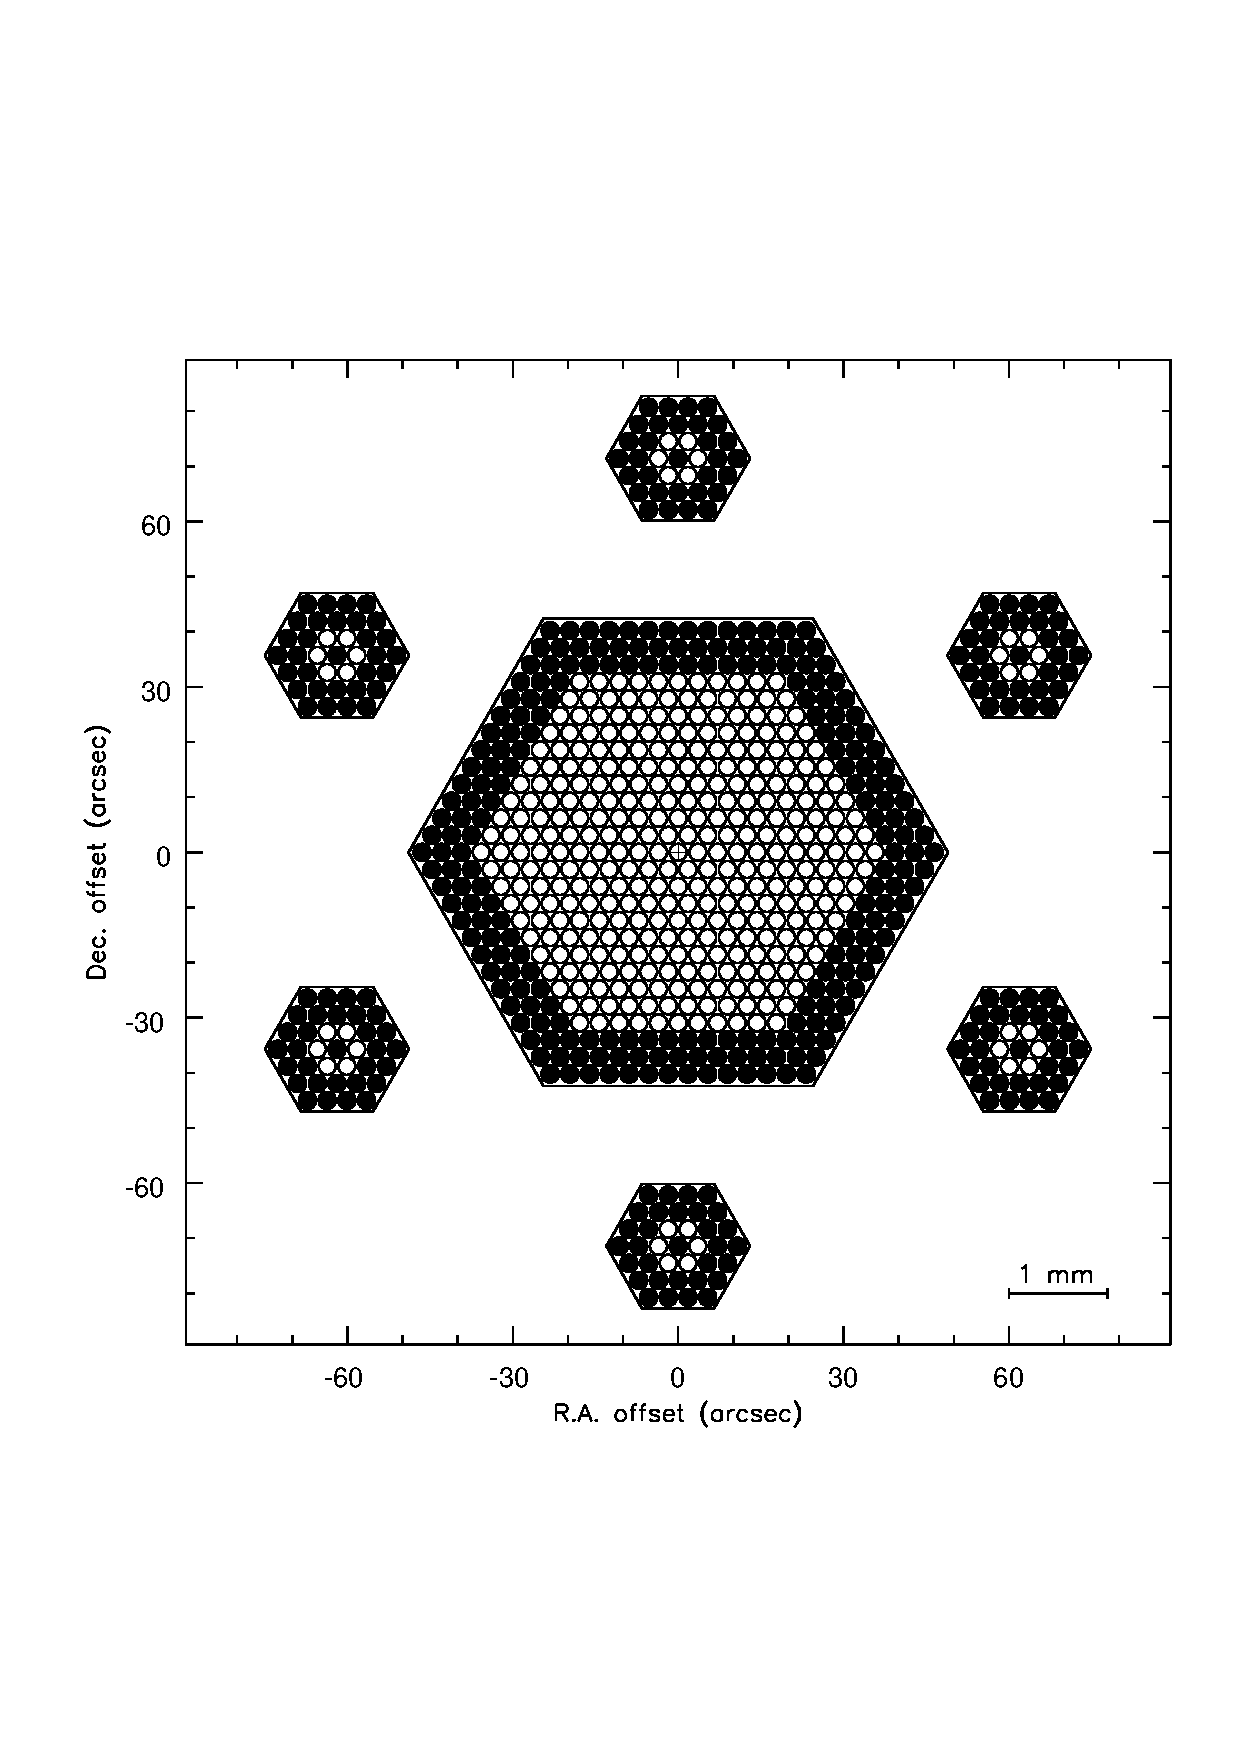
\includegraphics[width=0.7\textwidth]{figuras/Fig5.pdf}
    \caption[{\em Layout} do {\em bundle} de fibras do PPMAS/PPAK.]
    {Este é o esquema com o {\em bundle} hexagonal com as 331 fibras de
    observação e mais 36 de amostra de céu. Retirado de \citet{Verheijen2004},
    figura $5$.}
    \label{fig:BundlePPAK}
\end{figure}

Os objetos observados pelo CALIFA estão no universo local com $redshifts$ entre
$0.005 < z < 0.03$ e estão distribuídos em uma ampla variedade de tipos
morfologicos, massa em estrelas, condições do gas ionizante.

%***************************************************************%
%                                                               %
%                            PyCASSO                            %
%                                                               %
%***************************************************************%

\section{O {\em pipeline} PyCASSO}
\label{sec:CALePyC:PyCASSO}

% End of this chapter
